\section{クラスタリング実験}

\subsection{実験環境}
実験にはPython3.5を用い,
機械学習のライブラリとしてTensorFlowを用いてアルゴリズムを実装した.

\subsection{精度の評価}
クラスタリング精度の評価はPythonのライブラリであるscilit-learnを用い,以下の3項目により行う.
\begin{description}
  \item[ARI; Adjusted Rand Index, 調整ランド指数]~\\
    クラスタの正解ラベルに対してクラスタリング結果の一致度を評価する指標.1に近づくほどよい結果.
  \item[NMI; Normalized Mutual Information, 正規化相互情報量]~\\
    相互情報量を正規化した尺度.
  \item[Purity]~\\
    生成されたクラスタがどれだけ多数派で占められているかを表す尺度
\end{description}

\subsection{X-meansによるクラスタリング}
\subsubsection{2次元のクラスタリング}

まず,2次元のデータのクラスタリング結果を比較する.
2次元空間に分散$\sigma^2=1$のGauss分布により生成した,クラスタあたりのサンプル数を500として5つのクラスタを生成し,
対数尤度関数,BIC, AIC, cAICによりクラスタリングを行った.

\tablenum{table:2dim}に100回クラスタリングを行ったときの,推定されたクラスタ数,ARI, NMI, Purityの平均値および
クラスタ数の分散値を示す.
また,\figurenum{fig:2dim}に2次元空間におけるクラスタリングの例を示す.

\begin{table}[htb]
  \centering
  \caption{2次元空間におけるクラスタリング結果}
  \label{table:2dim}
  \begin{tabular}{|c|c|c|c|c|} \hline
    情報量規準 & クラスタ数(分散) & ARI & NMI & Purity \\\hline
    BIC & 4.58 (0.9836) & 0.84458792 & 0.88281495 & 0.84458792\\
    cAIC & 4.55 (0.6475) & 0.85329139 & 0.89992544 & 0.85329139\\
    AIC & 4.69 (3.8739) & 0.83642236 & 0.88147442 & 0.83642236\\
    対数尤度関数 & 5.32 (10.236) & 0.85699618 & 0.91572100 & 0.85699618\\\hline 
  \end{tabular}
\end{table}

\begin{figure}[htbp]
  \begin{minipage}{0.5\hsize}
    \begin{center}
      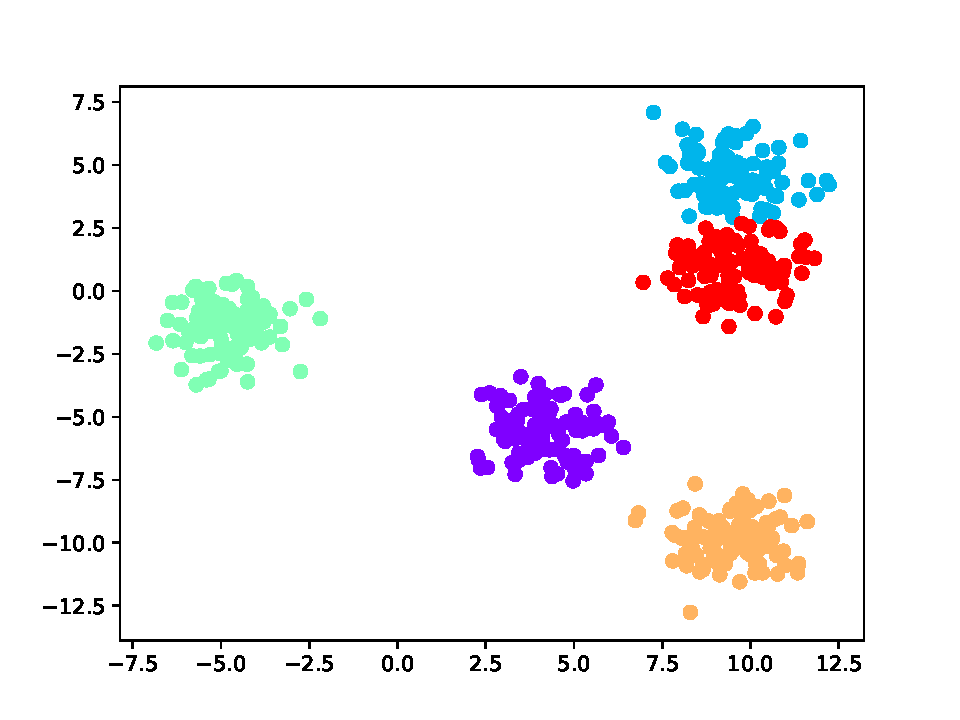
\includegraphics[width=0.9\linewidth]{./img/BIC_2.pdf}
      \caption{2次元空間のクラスタリング例}
      \label{fig:2dim}
    \end{center}
  \end{minipage}
  \begin{minipage}{0.5\hsize}
    \begin{center}
      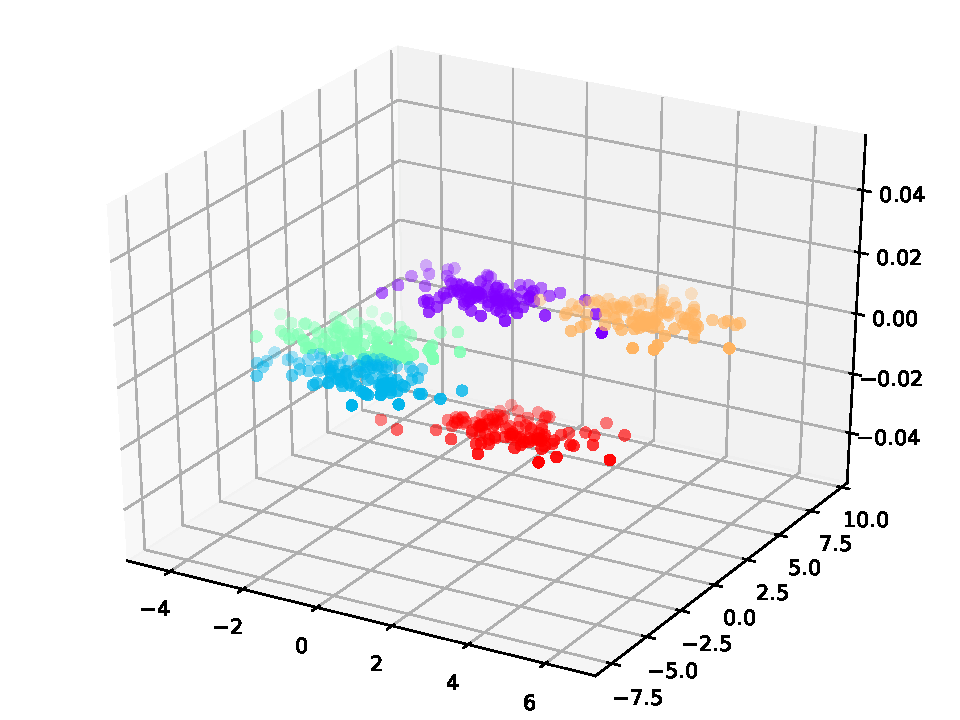
\includegraphics[width=0.9\linewidth]{./img/BIC_3.pdf}
      \caption{3次元空間のクラスタリング例}
      \label{fig:3dim}
    \end{center}
  \end{minipage}
\end{figure}

\subsubsection{3次元のクラスタリング}

3次元空間に分散$\sigma^2=1$のGauss分布により生成した,クラスタあたりのサンプル数を500として5つのクラスタを生成し,
対数尤度関数,BIC, AIC, cAICによりクラスタリングを行った.

\tablenum{table:3dim}に100回クラスタリングを行ったときの,推定されたクラスタ数,ARI,NMI,Purityの平均値および
クラスタ数の分散を示す.

また,\figurenum{fig:3dim}に2次元空間におけるクラスタリングの例を示す.

\begin{table}[htb]
  \centering
  \caption{3次元空間におけるクラスタリング結果}
  \label{table:3dim}
  \begin{tabular}{|c|c|c|c|c|} \hline
    情報量規準 & クラスタ数(分散) & ARI & NMI & Purity \\\hline
    BIC & 4.95 (0.0669) & 0.97179074 & 0.97913818 & 0.97179074\\
    cAIC & 4.92 (0.2313) & 0.96312702 & 0.97023920 & 0.96312702\\
    AIC & 4.88 (0.1443) & 0.95216819 & 0.96855698 & 0.95216819\\
    対数尤度関数 & 5.12 (4.1443) & 0.95731637 & 0.96541468 & 0.95731637\\\hline 
  \end{tabular}
\end{table}
